\section{张量分解}\label{chapter:tensor-decomposition}
处理高阶张量的计算代价很高，因为元素个数随张量的阶呈指数增长。为应对这一问题，张量分解应运而生，成为有力而高效的工具。
与矩阵分解类似，张量分解把一个高阶张量拆成阶数更低、元素更少的若干小分量，从而使计算更易处理。但矩阵秩的概念可以以多种方式推广到张量，每种推广都对应一种不同的因子化/分解模型。
本章介绍最广为人知的几种张量分解模型。
\subsection{并行因子/CP 分解（CANDECOMP/PARAFAC~Decomposition）}\label{sec:cp-decomposition}
$N$ 阶张量 $\At\in\RR^{d_1\times\cdots\times d_N}$ 的 CP 分解~\citep{hitchcock1927expression}把 $\At$ 分解为有限个秩一张量之和。等价地，它是 $R$ 个秩一张量的线性组合，其中 $R$ 称为该分解的秩：
$$\At = \sum_{r=1}^R \ab^{(r)}_1\outprod\dots\outprod\ab^{(r)}_N ,$$
其中对每个 $n\in [N]$，都有 $\ab^{(1)}_n,\dots,\ab^{(R)}_n\in\RR^{d_n}$。

把所有向量 $\ab^{(r)}_n$ 排成因子矩阵，
\[\Ab_1 = {\begin{pmatrix}
\ab^{(1)}_1 & \dots & \ab^{(R)}_1 \\
\end{pmatrix}}{\in\RR^{d_1\times R}}, \dots ,\Ab_N = {\begin{pmatrix}
\ab^{(1)}_N & \dots & \ab^{(R)}_N \\
\end{pmatrix}}{\in\RR^{d_N\times R}}, \]
CP 分解可简洁地记作 $\At = \CP{\Ab_1,\cdots,\Ab_N}$。

在张量网络中，CP 分解 $\At = \CP{\Ab,\Bb,\Cb}$ 表示为
$$
\begin{tikzpicture}[baseline=\baseline]
    \tikzset{tensor/.style = {minimum size = 0.5cm,shape = circle,thick,draw=black,inner sep = 0pt}, edge/.style   = {thick,line width=.4mm},every loop/.style={}}
    \def\y{0}
    \def\x{0}
    \node[tensor,fill=green!50!red!50!white] (A) at (\x,\y){\scalebox{0.85}{$\At$}};
    \draw[edge] (\x+0.25,\y) -- (\x+0.6,\y)  node [midway,above] {\scalebox{0.7}{\dimcolor{$d_2$}}};
    \draw[edge] (\x-0.25,\y) -- (\x-0.6,\y)  node [midway,above] {\scalebox{0.7}{\dimcolor{$d_1$}}};
    \draw[edge] (\x,\y-0.25) -- (\x,\y-0.7)  node [midway,left] {\scalebox{0.7}{\dimcolor{$d_3$}}};
    \end{tikzpicture}
=
\begin{tikzpicture}[baseline=\baseline]
    \tikzset{tensor/.style = {minimum size = 0.5cm,shape = circle,thick,draw=black,inner sep = 0pt}, edge/.style   = {thick,line width=.4mm},every loop/.style={}}
    \def\y{0}
    \def\x{0}
  \node[tensor,fill=red!50!white] (A) at (\x,\y){\scalebox{0.85}{$\Ab$}};
  \node[tensor,fill=blue!50!white] (B) at (\x+1,\y){$\Bb$};
   \node[tensor,fill=blue!20!white] (C) at (\x+2,\y){$\Cb$};
    \draw  node[fill = black,circle,inner sep=0pt,minimum size=4pt] (m) at (\x+1,\y+0.7) {};
    \draw[edge] (A) -- (m);
    \node[draw=none] () at (\x+0.4,\y+0.5) {\scalebox{0.7}{\dimcolor{$R$}}};
    \draw[edge] (B) -- (m) node [midway,left=-0.09cm] {\scalebox{0.7}{\dimcolor{$R$}}};
    \draw[edge] (C) -- (m);
    \node[draw=none] () at (\x+1.6,\y+0.5) {\scalebox{0.7}{\dimcolor{$R$}}};
    \draw[edge](A) -- (\x,\y-0.7)node [midway,left] {\edgelabel{$d_1$}};
    \draw[edge](B) -- (\x+1,\y-0.7)node [midway,left] {\edgelabel{$d_2$}};
    \draw[edge](C) -- (\x+2,\y-0.7)node [midway,left] {\edgelabel{$d_3$}};
\end{tikzpicture},
$$
其中黑点是第~\ref{sec:copy-tensor}~节引入的三阶复制张量。事实上，有
\begin{align*}
    \left(\begin{tikzpicture}[baseline=\baseline]
    \tikzset{tensor/.style = {minimum size = 0.5cm,shape = circle,thick,draw=black,inner sep = 0pt}, edge/.style   = {thick,line width=.4mm},every loop/.style={}}
    \def\y{0}
    \def\x{0}
  \node[tensor,fill=red!50!white] (A) at (\x,\y){\scalebox{0.85}{$\Ab$}};
  \node[tensor,fill=blue!50!white] (B) at (\x+1,\y){$\Bb$};
   \node[tensor,fill=blue!20!white] (C) at (\x+2,\y){$\Cb$};
    \draw  node[fill = black,circle,inner sep=0pt,minimum size=4pt] (m) at (\x+1,\y+0.7) {};
    \draw[edge] (A) -- (m);
    \node[draw=none] () at (\x+0.4,\y+0.5) {\scalebox{0.7}{\dimcolor{$R$}}};
    \draw[edge] (B) -- (m) node [midway,left=-0.09cm] {\scalebox{0.7}{\dimcolor{$R$}}};
    \draw[edge] (C) -- (m);
    \node[draw=none] () at (\x+1.6,\y+0.5) {\scalebox{0.7}{\dimcolor{$R$}}};
    \draw[edge](A) -- (\x,\y-0.7);
    \draw[edge](B) -- (\x+1,\y-0.7);
    \draw[edge](C) -- (\x+2,\y-0.7);
\end{tikzpicture}\right)_{ijk} 
&= \sum_{r_1=1}^R\sum_{r_2=1}^R\sum_{r_3=1}^R\delta_{r_1r_2r_3}\Ab_{ir_1}\Bb_{jr_2}\Cb_{kr_3}
=
\sum_{r=1}^R\Ab_{ir}\Bb_{jr}\Cb_{kr}\\
&=
\sum_{r=1}^R(\ab_r)_i(\bb_r)_j(\cbb_r)_k 
=
\sum_{r=1}^R(\ab_r\outprod\bb_r\outprod\cbb_r)_{ijk}\\
&=
\left(\sum_{r=1}^R\ab_r\outprod\bb_r\outprod\cbb_r\right)_{ijk}
\end{align*}
\paragraph{张量的 CP 秩}
张量秩最基本也是最早的概念是 CP 秩，最早由~\citep{hitchcock1927expression}提出。张量的 CP 秩定义为：把该张量表示为若干秩一张量之和所需的最少项数。\footnote{注意本文术语中「CP 分解的秩」与「张量的 CP 秩」有一细微差别：前者的秩指形如 $\At = \sum_{r=1}^R \ab^{(r)}_1\outprod\dots\outprod\ab^{(r)}_N$ 的分解中求和项的个数，而张量 $\At$ 的 CP 秩是使这样的分解存在的最小的 $R$。因此，若 $\At$ 有一个秩 $R$ 的 CP 分解，其 CP 秩至多为 $R$，也可能更小。}
尽管这一定义与矩阵秩的定义相似，张量秩的性质却与之大不相同。从计算的角度看，一个关键区别在于：与矩阵秩不同，不存在能在多项式时间内确定张量 CP 秩的算法。事实上，计算张量的秩是 NP 难问题~\citep{hillar2013most}。
张量秩还有若干变体，每个变体都与某种特定的张量分解相对应。随着本章的推进，我们会介绍其中几种不同的秩。


\begin{remark}
\newcommand*{\horzbar}{\rule[.5ex]{2.5ex}{0.5pt}}
这里列出 CP 秩与 CP 分解的一些有趣性质。
\begin{enumerate}
\item 
由定理~\ref{thm: matricization-rank}与命题~\ref{prop:copy.tensor}~（第 3 条）可知：若张量 $\At$ 存在秩 $R$ 的 CP 分解，则它的所有矩阵化的秩都不超过 $R$：
\begin{proposition}
    若 $\At = \CP{\Ab_1,\cdots, \Ab_N}$ 是 $\At$ 的一个秩 $R$ 的 CP 分解，则对任意 $I\subset [N]$ 都有 $\rank(\At_{(I)}) \leq R$。
\end{proposition}
下面的张量网络以四阶张量 $\At = \CP{\Ab_1,\Ab_2,\Ab_3, \Ab_N}$ 沿其前两个模的矩阵化为例，说明了这一结论。
\begin{align*}
    \left(
    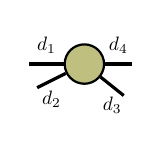
\begin{tikzpicture}[baseline=-0.5ex]
    \tikzset{tensor/.style = {minimum size = 0.5cm,shape = circle,thick,draw=black,inner sep = 0pt}, edge/.style = {thick,line width=.4mm},every loop/.style={}}
    \def\x{6}
    \def\y{0}   \node[tensor,fill=green!50!red!50!white] (T) at (\x+1,\y) {$\At$};
    \draw[edge] (T) -- (\x+0.3,0) node [midway,above] {\scalebox{0.7}{\dimcolor{$d_1$}}};
    \draw[edge] (T) -- (\x+1.6,0) node [midway,above] {\scalebox{0.7}{\dimcolor{$d_4$}}};;
    \draw[edge] (T) -- (\x+0.4,-0.3) node [midway, below] {\scalebox{0.7}{\dimcolor{$d_2$}}};
    \draw[edge] (T) -- (\x+1.5,-0.4)node [midway, below] {\scalebox{0.7}{\dimcolor{$d_3$}}};
\end{tikzpicture}\right)_{(\{1,2\})}
&=
\left(\begin{tikzpicture}[baseline=\baseline]
    \tikzset{tensor/.style = {minimum size = 0.5cm,shape = circle,thick,draw=black,inner sep = 0pt}, edge/.style   = {thick,line width=.4mm},every loop/.style={}}
    \def\y{0}
    \def\x{0}
  \node[tensor,fill=red!50!white] (A) at (\x,\y){\scalebox{0.85}{$\Ab_1$}};
  \node[tensor,fill=blue!50!white] (B) at (\x+1,\y){$\Ab_2$};
   \node[tensor,fill=red!20!white] (C) at (\x+2,\y){$\Ab_3$};
    \node[tensor,fill=blue!20!white] (D) at (\x+3,\y){$\Ab_4$};
    \draw  node[fill = black,circle,inner sep=0pt,minimum size=4pt] (m) at (\x+1.5,\y+0.7) {};
    \draw[edge] (A) -- (m)node [midway, above] {\scalebox{0.7}{\dimcolor{$R$}}} ;
    \draw[edge] (B) -- (m);
    \draw[edge] (C) -- (m);
    \draw[edge] (D) -- (m)node [midway, above] {\scalebox{0.7}{\dimcolor{$R$}}};
    \draw[edge](A) -- (\x,\y-0.7)node [midway,left] {\scalebox{0.7}{\dimcolor{$d_1$}}};
    \draw[edge](B) -- (\x+1,\y-0.7)node [midway,left] {\scalebox{0.7}{\dimcolor{$d_2$}}};
    \draw[edge](C) -- (\x+2,\y-0.7)node [midway,left] {\scalebox{0.7}{\dimcolor{$d_3$}}};
    \draw[edge](D) -- (\x+3,\y-0.7) node [midway,left] {\scalebox{0.7}{\dimcolor{$d_4$}}};
\end{tikzpicture}\right)_{(\{1,2\})}\\
&=
\begin{tikzpicture}[baseline=\baseline]
    \tikzset{tensor/.style = {minimum size = 0.5cm,shape = circle,thick,draw=black,inner sep = 0pt}, edge/.style   = {thick,line width=.4mm},every loop/.style={}}
    \def\y{0}
    \def\x{0}
  \node[tensor,fill=red!50!white] (A) at (\x,\y){\scalebox{0.85}{$\Ab_1$}};
  \node[tensor,fill=blue!50!white] (B) at (\x+1,\y){$\Ab_2$};
   \node[tensor,fill=red!20!white] (C) at (\x+2,\y){$\Ab_3$};
    \node[tensor,fill=blue!20!white] (D) at (\x+3,\y){$\Ab_4$};
    \draw  node[fill = black,circle,inner sep=0pt,minimum size=4pt] (m1) at (\x+0.5,\y+0.7) {};
    \draw  node[fill = black,circle,inner sep=0pt,minimum size=4pt] (m2) at (\x+2.5,\y+0.7) {};
    \draw[edge](A) -- (\x,\y-0.65) -- (\x+0.5,\y-0.65) -- (\x+0.5,\y-1);
    \draw[edge](B) -- (\x+1,\y-0.65) -- (\x+0.6,\y-0.65) -- (\x+0.6,\y-1);
    \draw[edge](C) -- (\x+2,\y-0.65) -- (\x+2.5,\y-0.65) -- (\x+2.5,\y-1);
    \draw[edge](D) -- (\x+3,\y-0.65) -- (\x+2.6,\y-0.65) -- (\x+2.6,\y-1);
    \node[draw=none] at (\x+0.55,\y-1.15){\scalebox{0.7}{\dimcolor{$d_1d_2$}}};
    \node[draw=none] at (\x+2.55,\y-1.15){\scalebox{0.7}{\dimcolor{$d_3d_4$}}};
    \draw[dotted] (\x+1.5,\y+1.5) -- (\x+1.5,\y-0.7);
    \draw[edge](A) -- (m1)node [midway,left] {\scalebox{0.7}{\dimcolor{$R$}}};;
    \draw[edge](B) -- (m1)node [midway,right] {\scalebox{0.7}{\dimcolor{$R$}}};
    \draw[edge](C) -- (m2)node [midway,left] {\scalebox{0.7}{\dimcolor{$R$}}};
    \draw[edge](D) -- (m2)node [midway,right] {\scalebox{0.7}{\dimcolor{$R$}}};
    \draw[edge](m1)--(m2)node [near start, above] {\scalebox{0.7}{\dimcolor{$R$}}};
\end{tikzpicture}.
\end{align*}
\item  张量 $\At \in \RR^{d_1\times \cdots \times d_N}$ 的 CP 秩有一个容易得到的上界~\citep{kolda2009tensor}
$$\cprank(\At)\leq \min_{n\in [N]} \prod_{i\neq n} d_i.$$
\item 对二阶张量 $\Ab\in\RR^{d_1\times d_2}$，CP 秩恰好对应经典的矩阵秩概念。
\item CP 分解 $\At = \CP{\Ab,\Bb,\Cb}$ 可用克罗内克 $\delta$ 写为
$$\At_{i,j,k} = \sum_{r_1,r_2,r_3}\delta_{r_1,r_2,r_3}\Ab_{i,r_1}\Bb_{j,r_2}\Cb_{k,r_3},$$
也可借助模 $n$ 乘积写成（见~\ref{par:mode-n-tensor-product}）
$$\At = \It\ttm{1}\Ab\ttm{2}\Bb\ttm{3}\Cb$$
其中 $\It$ 为三阶复制张量。
\item 二阶张量（矩阵）的秩在域 $\RR$ 与 $\CC$ 上是相同的。但对高阶张量（阶数 $N\geq3$ 的 $N$ 阶张量），秩会随分解所用的域而改变~\citep{kruskal1989rank}。
\item 对一个 $N$ 阶、每维长度均为 $d$ 的张量（$d_1 = \dots = d_N = d$），其 CP 分解的参数个数为 $NdR$，而完整张量需要 $d^N$ 个参数。若 $R$ 很小，参数个数便可大幅减少。
\end{enumerate}
\end{remark}
下面的命题说明：张量 CP 分解的模 $n$ 矩阵化可以用 Khatri-Rao 积来表达。
\begin{proposition}
设 $\At\in\RR^{d_1\times d_2\times\dots\times d_N}$。若 $\At=\CP{\Ab_1,\Ab_2,\dots,\Ab_N}$，则
$$\At_{(n)}=\Ab_n\left(\Ab_1\krao\dots\krao\Ab_{(n-1)}\krao\Ab_{(n+1)}\krao\dots\krao\Ab_N\right)^\ts.$$
\begin{proof}
取 $N=3$ 且 $n=1$，
\begin{align*}
\At_{(1)}
&=
\left(\begin{tikzpicture}[baseline=\baseline]
    \tikzset{tensor/.style = {minimum size = 0.5cm,shape = circle,thick,draw=black,inner sep = 0pt}, edge/.style  = {thick,line width=.4mm},every loop/.style={}}
    \def\y{0}
    \def\x{0}
    \node[tensor,fill=green!50!red!50!white] (At) at (\x,\y){\scalebox{0.85}{$\At$}};
    \draw[edge] (\x+0.25,\y) -- (\x+0.6,\y)  node [midway,above] {\scalebox{0.7}{\dimcolor{$d_2$}}};
    \draw[edge] (\x-0.25,\y) -- (\x-0.6,\y)  node [midway,above] {\scalebox{0.7}{\dimcolor{$d_1$}}};
    \draw[edge] (\x,\y-0.25) -- (\x,\y-0.7)  node [midway,left] {\scalebox{0.7}{\dimcolor{$d_3$}}};
    \end{tikzpicture}\right)_{(1)}
=
\left(\begin{tikzpicture}[baseline=\baseline]
    \tikzset{tensor/.style = {minimum size = 0.5cm,shape = circle,thick,draw=black,inner sep = 0pt}, edge/.style   = {thick,line width=.4mm},every loop/.style={}}
    \def\y{0}
    \def\x{0}
  \node[tensor,fill=red!50!white] (A1) at (\x,\y){\scalebox{0.85}{$\Ab_1$}};
  \node[tensor,fill=blue!50!white] (A2) at (\x+1,\y){$\Ab_2$};
   \node[tensor,fill=blue!20!white] (A3) at (\x+2,\y){$\Ab_3$};
    \draw  node[fill = black,circle,inner sep=0pt,minimum size=4pt] (m) at (\x+1,\y+1) {};
    \draw[edge] (A1) -- (m) node [midway,left] {\scalebox{0.7}{\dimcolor{$R$}}};
    \draw[edge] (A2) -- (m)node [midway,left=-0.05cm] {\scalebox{0.7}{\dimcolor{$R$}}};
    \draw[edge] (A3) -- (m)node [midway,right] {\scalebox{0.7}{\dimcolor{$R$}}};
    \draw[edge](A1) -- (\x,\y-0.7)node [midway,left] {\edgelabel{$d_1$}};
    \draw[edge](A2) -- (\x+1,\y-0.7)node [midway,left] {\edgelabel{$d_2$}};
    \draw[edge](A3) -- (\x+2,\y-0.7)node [midway,left] {\edgelabel{$d_3$}};
\end{tikzpicture}\right)_{(1)}\\
&=
\begin{tikzpicture}[baseline=\baseline]
    \tikzset{tensor/.style = {minimum size = 0.5cm,shape = circle,thick,draw=black,inner sep = 0pt}, edge/.style   = {thick,line width=.4mm},every loop/.style={}}
    \def\y{0}
    \def\x{0}
    \node[tensor,fill=green!50!red!50!white] (At) at (\x,\y){\scalebox{0.85}{$\At$}};
    \draw[edge] (\x-0.25,\y) -- (\x-0.6,\y)  node [midway,above] {\scalebox{0.7}{\dimcolor{$d_1$}}};
    \draw[edge] (\x+0.2,\y+0.15) -- (\x+0.5,\y+0.15)-- (\x+0.5,\y+0.05) -- (\x+1,\y+0.05) node [midway,above]
    {\scalebox{0.7}{\dimcolor{$d_2$}}};
    \draw[edge] (\x+0.2,\y-0.15) -- (\x+0.5,\y-0.15)-- (\x+0.5,\y-0.05)-- (\x+1,\y-0.05) node [midway,below]
    {\scalebox{0.7}{\dimcolor{$d_3$}}};
    \end{tikzpicture}
=
\begin{tikzpicture}[baseline=\baseline]
    \tikzset{tensor/.style = {minimum size = 0.5cm,shape = circle,thick,draw=black,inner sep = 0pt}, edge/.style   = {thick,line width=.4mm},every loop/.style={}}
    \def\y{0}
    \def\x{0}
    \node[tensor,fill=red!50!white] (A1) at (\x,\y){\scalebox{0.85}{$\Ab_1$}};
    \node[tensor,fill=blue!50!white] (A2) at (\x+1.7,\y+0.7){$\Ab_2$};
    \node[tensor,fill=blue!20!white] (A3) at (\x+1.7,\y-0.7){$\Ab_3$};
    \draw  node[fill = black,circle,inner sep=0pt,minimum size=4pt] (m) at (\x+1,\y) {};
    \draw[edge] (A1) -- (m) node [very near end,above] {\scalebox{0.7}{\dimcolor{$R$}}};
    \draw[edge] (A2) -- (m);
    \draw[edge] (A3) -- (m);
    \draw[edge] (A1) -- (\x-0.7,\y) node [midway,above] {\scalebox{0.7}{\dimcolor{$d_1$}}};
    \draw[edge] (A2) -- (\x+2.5,\y+0.7) -- (\x+2.5,\y+0.05)-- (\x+3,\y+0.05) node [midway,above]
    {\scalebox{0.7}{\dimcolor{$d_2$}}};
    \draw[edge] (A3) -- (\x+2.5,\y-0.7) -- (\x+2.5,\y-0.05) -- (\x+3,\y-0.05) node [midway,below]
    {\scalebox{0.7}{\dimcolor{$d_3$}}};
    \end{tikzpicture}
=
\Ab_1(\Ab_2\krao\Ab_3)^\ts.
\end{align*}
\end{proof}
\end{proposition}

